\documentclass[main.tex]{subfiles}
%\usepackage{functions}
\begin{document}
%%%%%%%%%%%%%%%%%%%%%%%%%%%%%%%%%%%%
\pgfkeys{/pgf/fpu=true}
%%%%%%%%%%%%%%%%%%%%%%%%%%%%%%%%%%%% Define Constant for pgf
%\pgfmathparse{} %
%\edef\Gconst{\pgfmathresult}

\chapter{Betelgeuse spectra etc}

\section{Schema dell'esperienza}

\subsection{Materiali}

\begin{itemize}
\item ponte a T doppio: \SI{4700}{\pico\farad}//\SI{4700}{\pico\farad}, \SI{82}{\ohm} (argento-nero rosso); \SI{221}{\pico\farad}//\SI{39}{\pico\farad}, \SI{1}{\kilo\ohm} (marrone-nero-rosso).
\end{itemize}

\subsection{Ponti a T.}
La condizione di isolamento \'e verificata per $R=\frac{1}{\omega C}$.
\begin{itemize}
\item Ponte a T doppio I.
\begin{figure}[!ht]\centering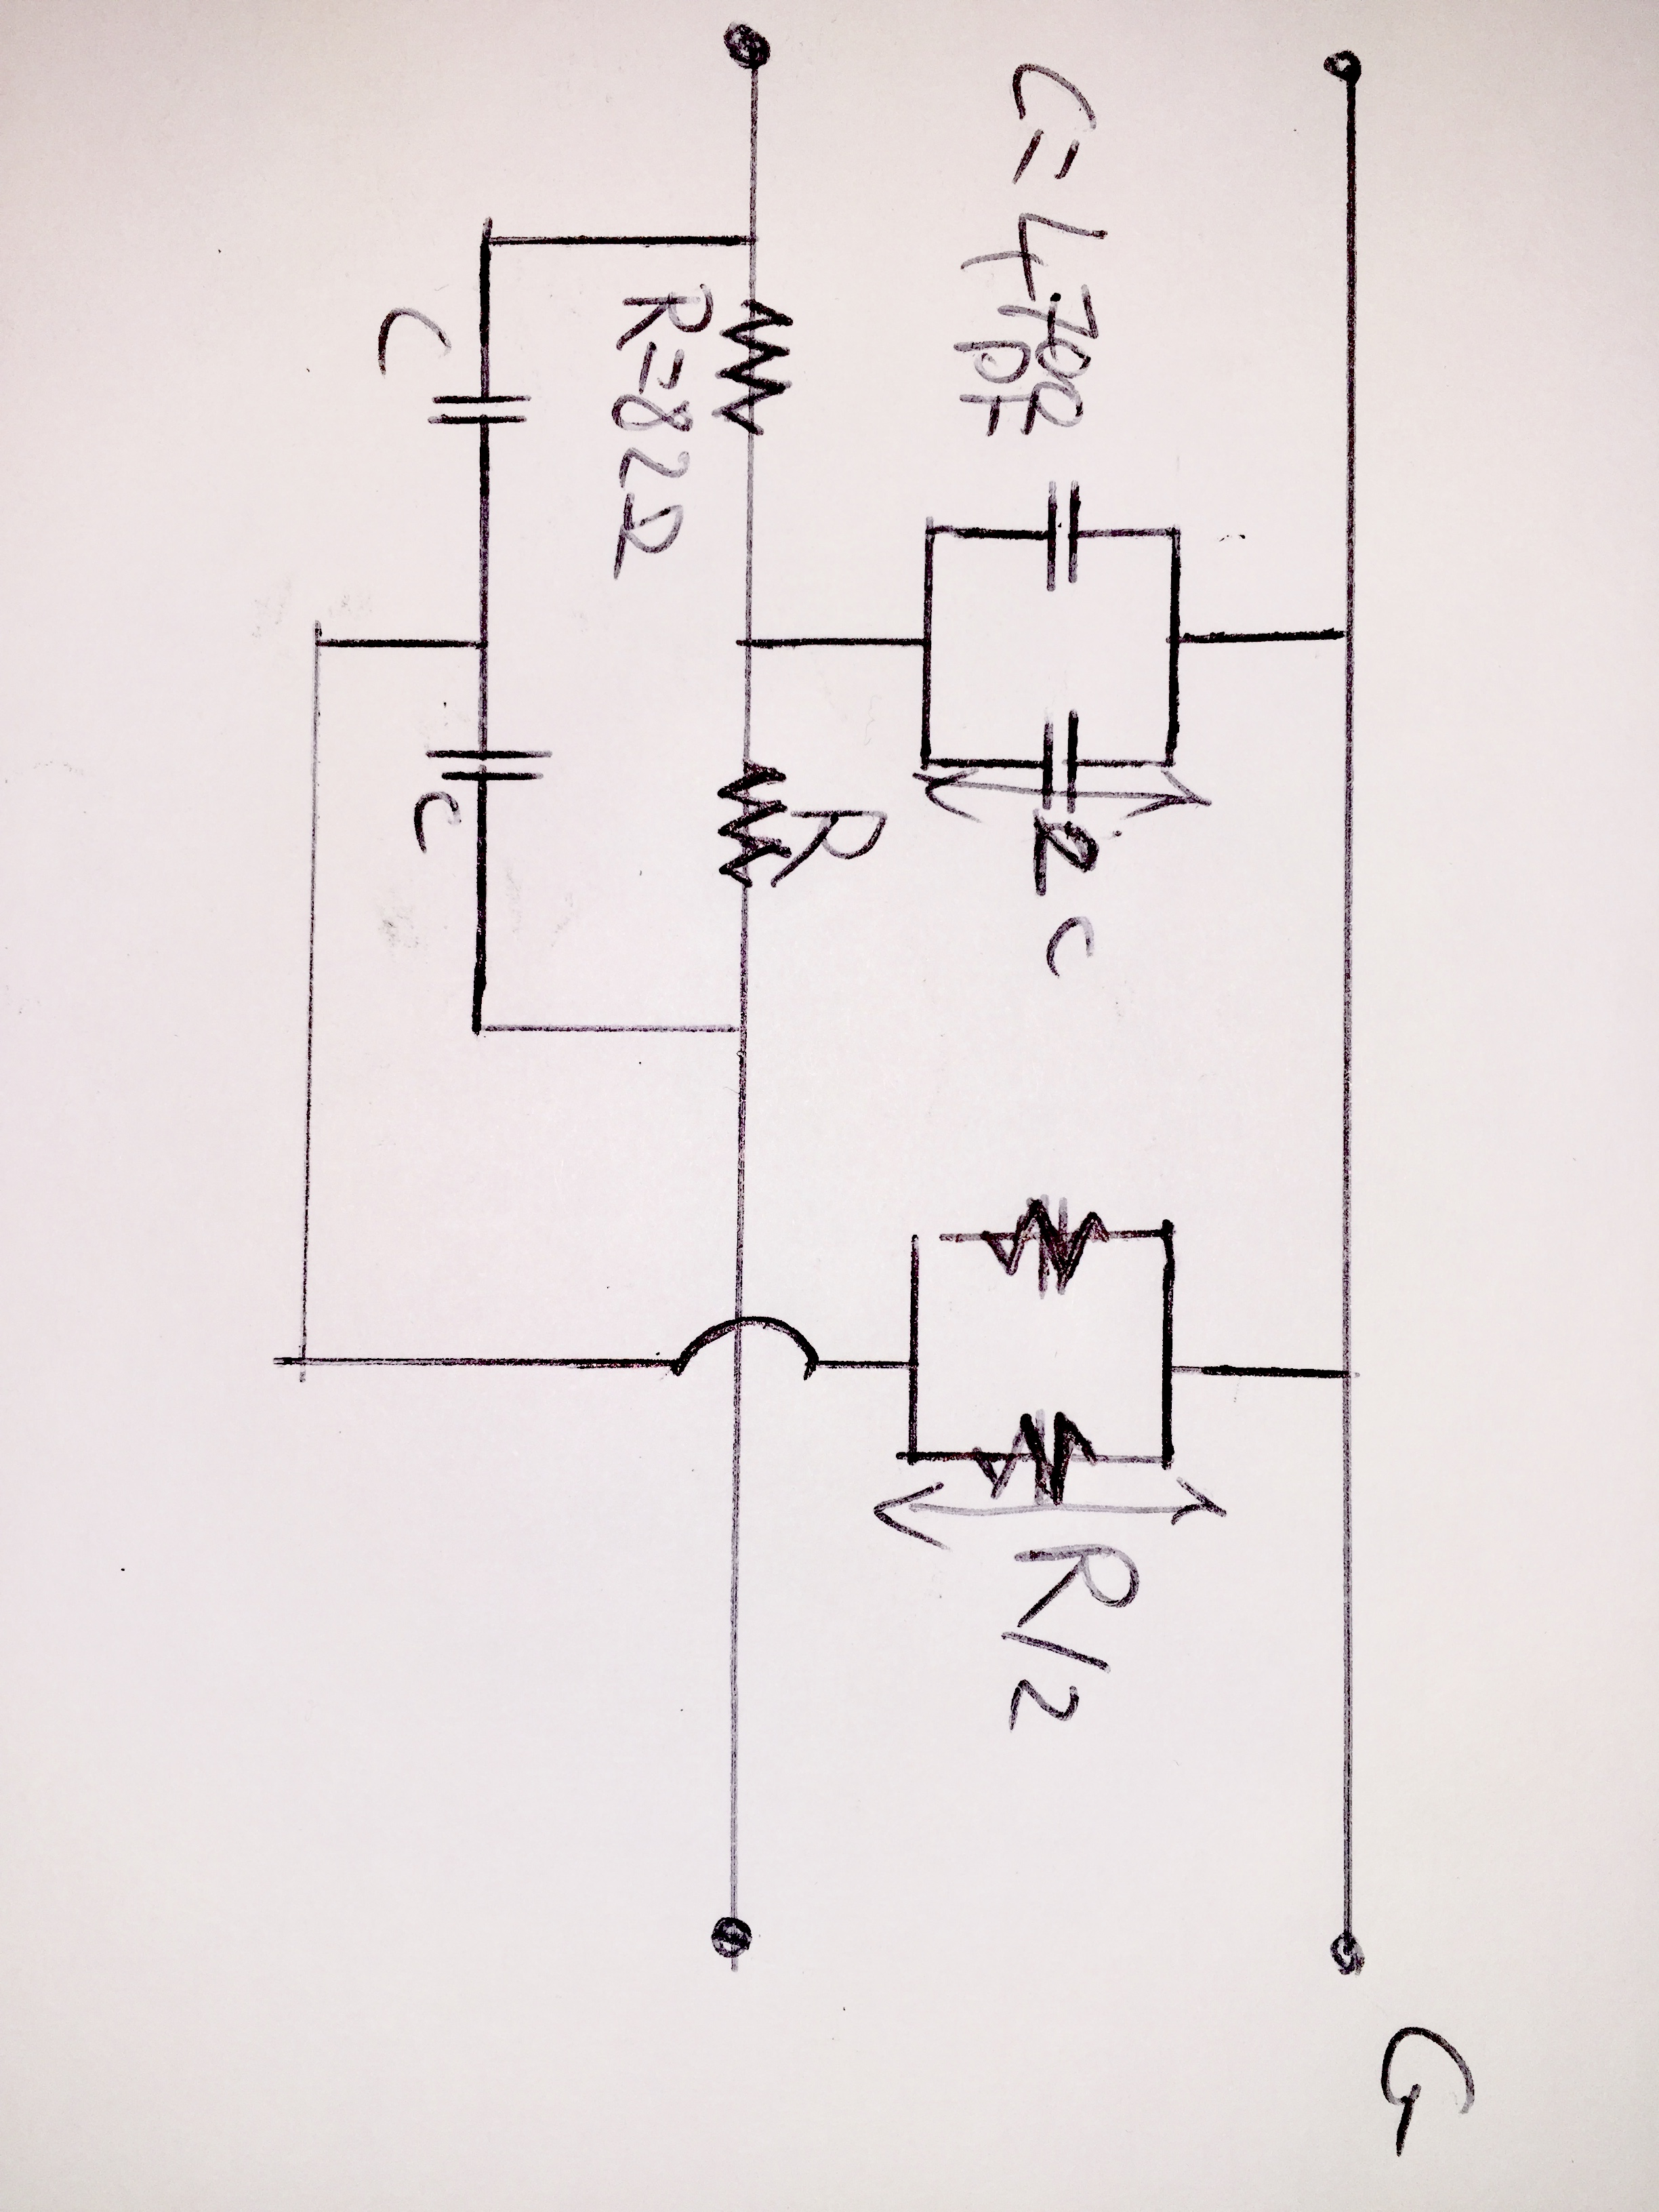
\includegraphics[trim={0cm 0cm 0 0},angle=90,clip, keepaspectratio,width=0.6\textwidth]{doppioT1}\caption{Ponte a T doppio I.}\label{fig:T1}\end{figure}
\edef\RT{82}   %reistenza grigio rosso nero
\edef\CT{4700*(10)^(-12)}   %capacita 4700
$\nu_{Zmax}=\pgfmathparse{((\CT*\RT)^(-1))/(2*pi)}\pgfmathprintnumber{\pgfmathresult}\si{\hertz}$ determinato usando il valore nominale degli elementi. Il valore determinato al minimo del coefficiente di trasmissione \'e \SI{415}{\kilo\hertz}.

\item Ponte a T doppio II.
\begin{figure}[!ht]\centering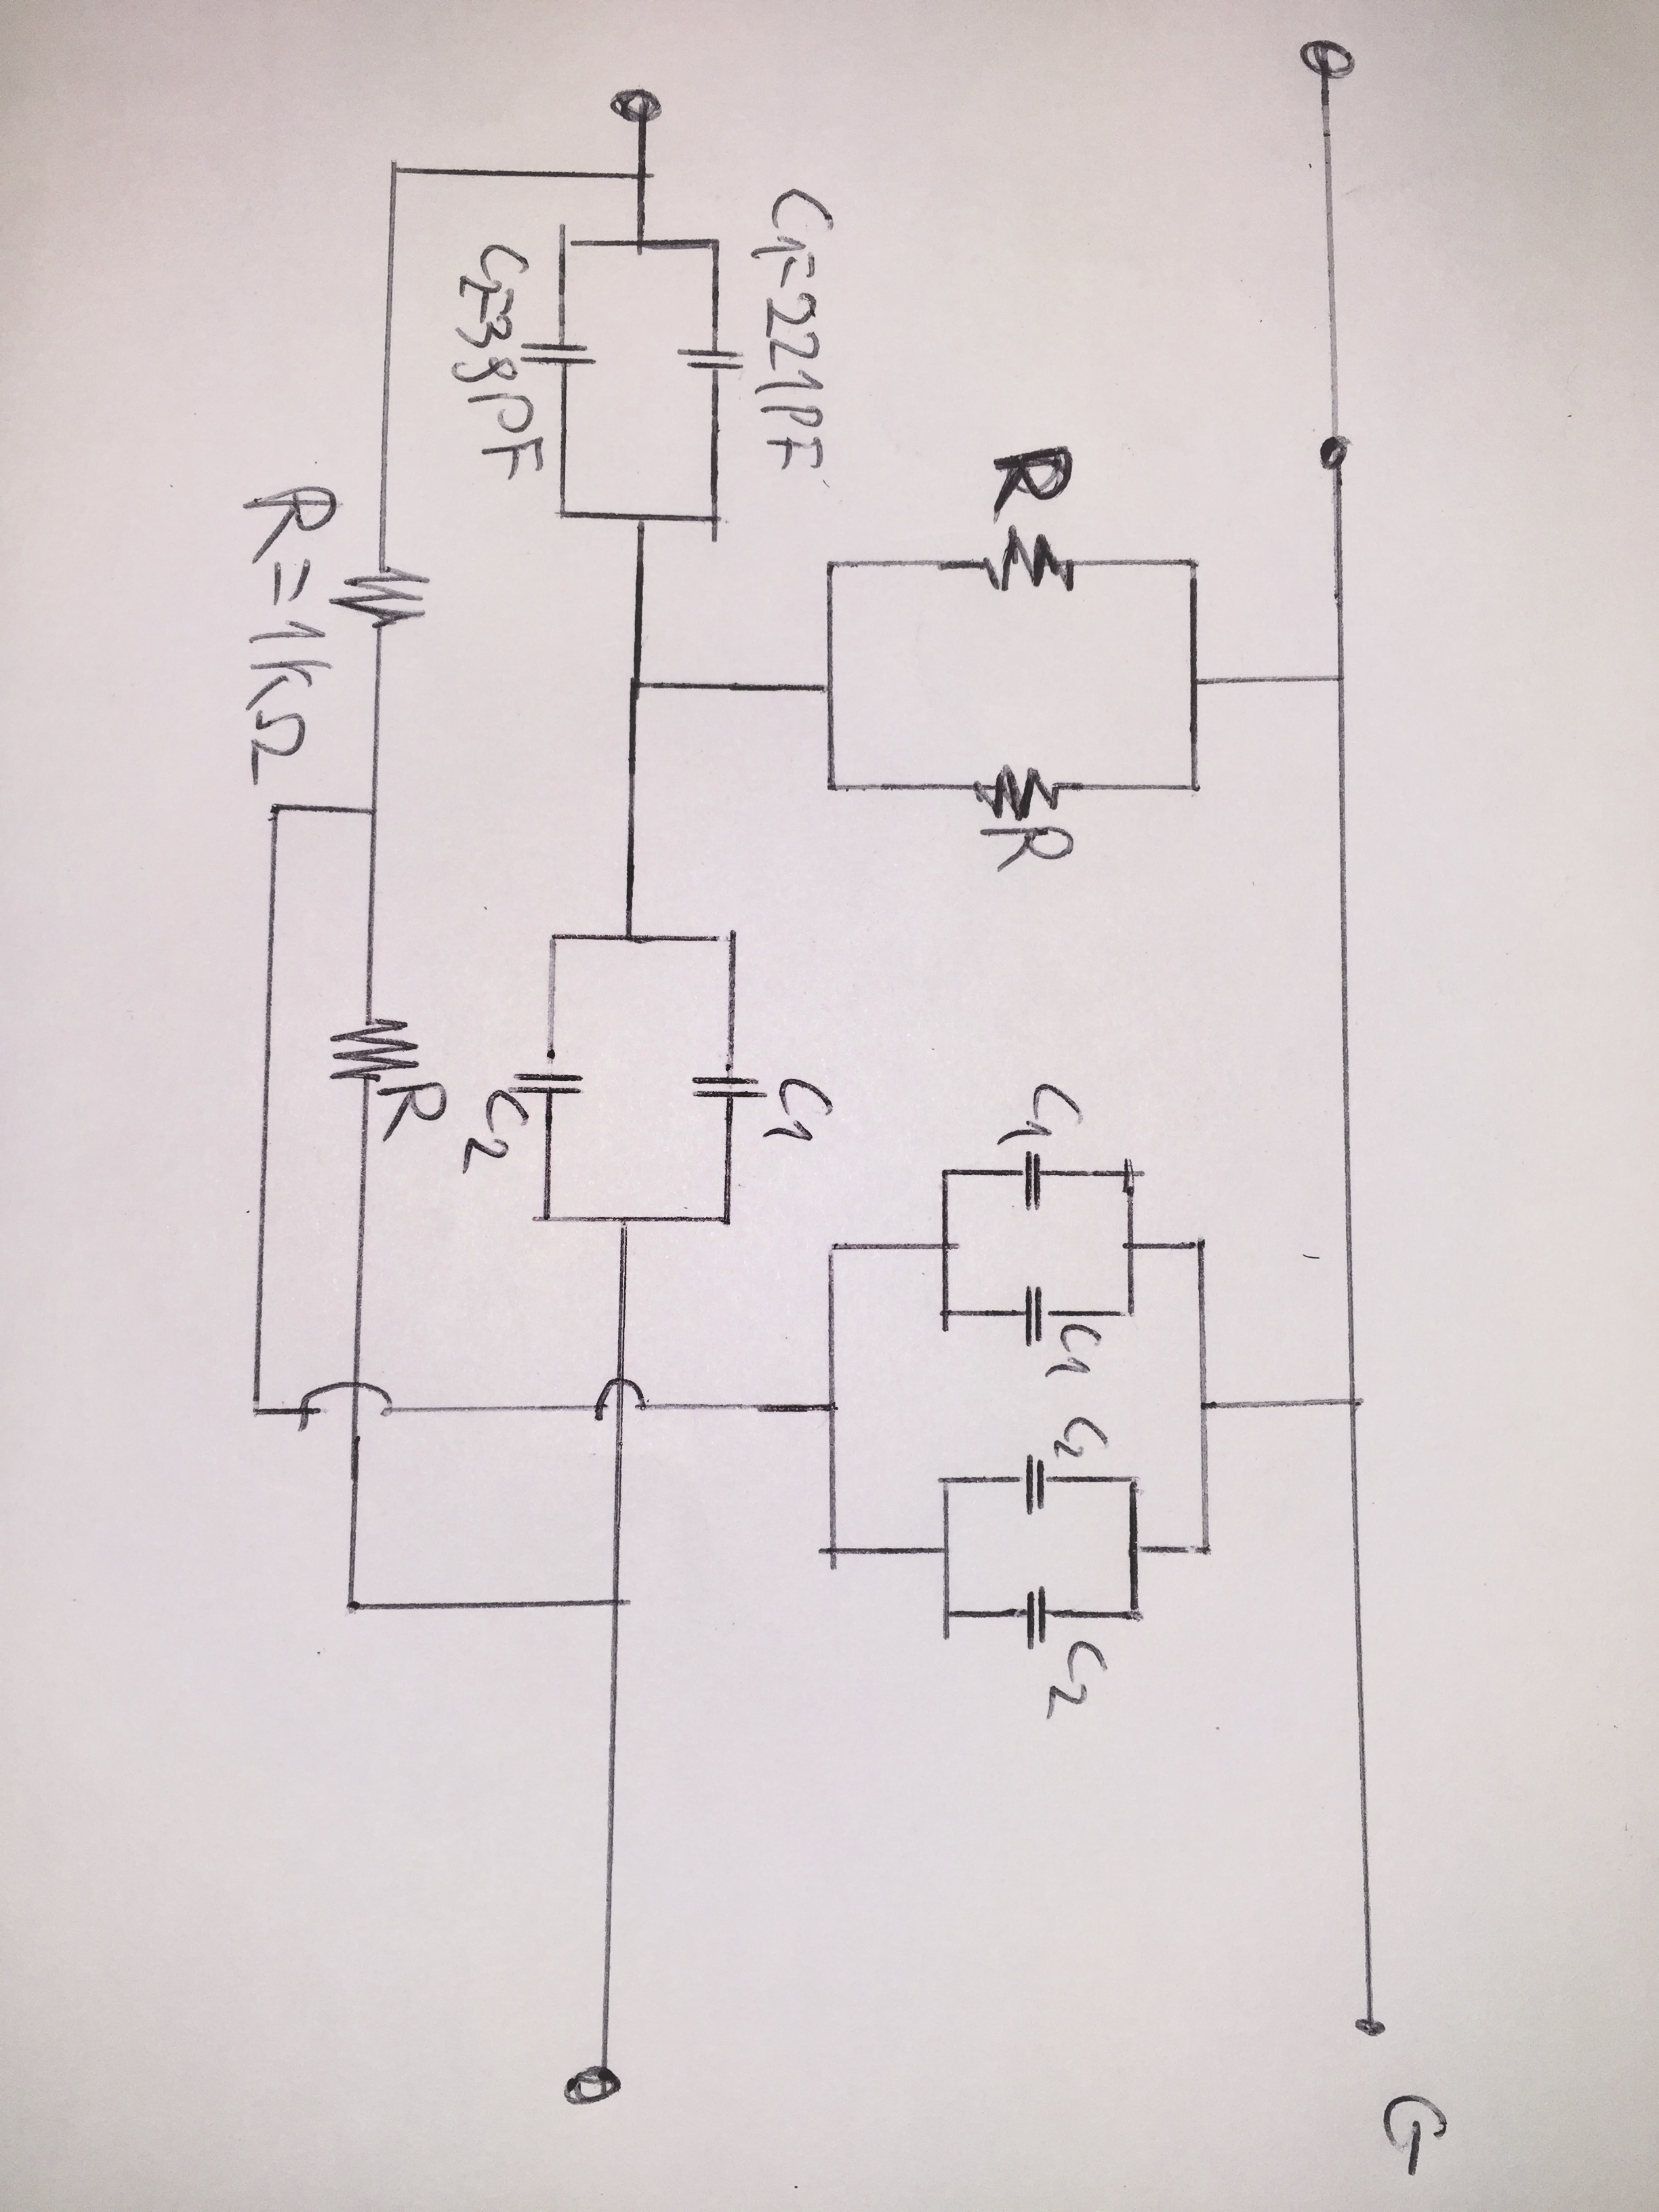
\includegraphics[trim={0cm 0cm 0 0},clip,angle=90,keepaspectratio,width=0.6\textwidth]{doppioT2}\caption{Ponte a T doppio II.}\label{fig:T2}\end{figure}
\edef\RT{1000}   %reistenza marrone nero rosso
\edef\CT{(39+221)*10^(-12)}   %capacita 39//221
$\nu_{Zmax}=\pgfmathparse{((\CT*\RT)^(-1))/(2*pi)}\pgfmathprintnumber{\pgfmathresult}\si{\hertz}$ determinato usando il valore nominale degli elementi. Il valore determinato al minimo del coefficiente di trasmissione \'e \SI{620}{\kilo\hertz}.

\end{itemize}

\subsection{Probe NMR}
\begin{wrapfigure}[10]{l}{0.5\textwidth} 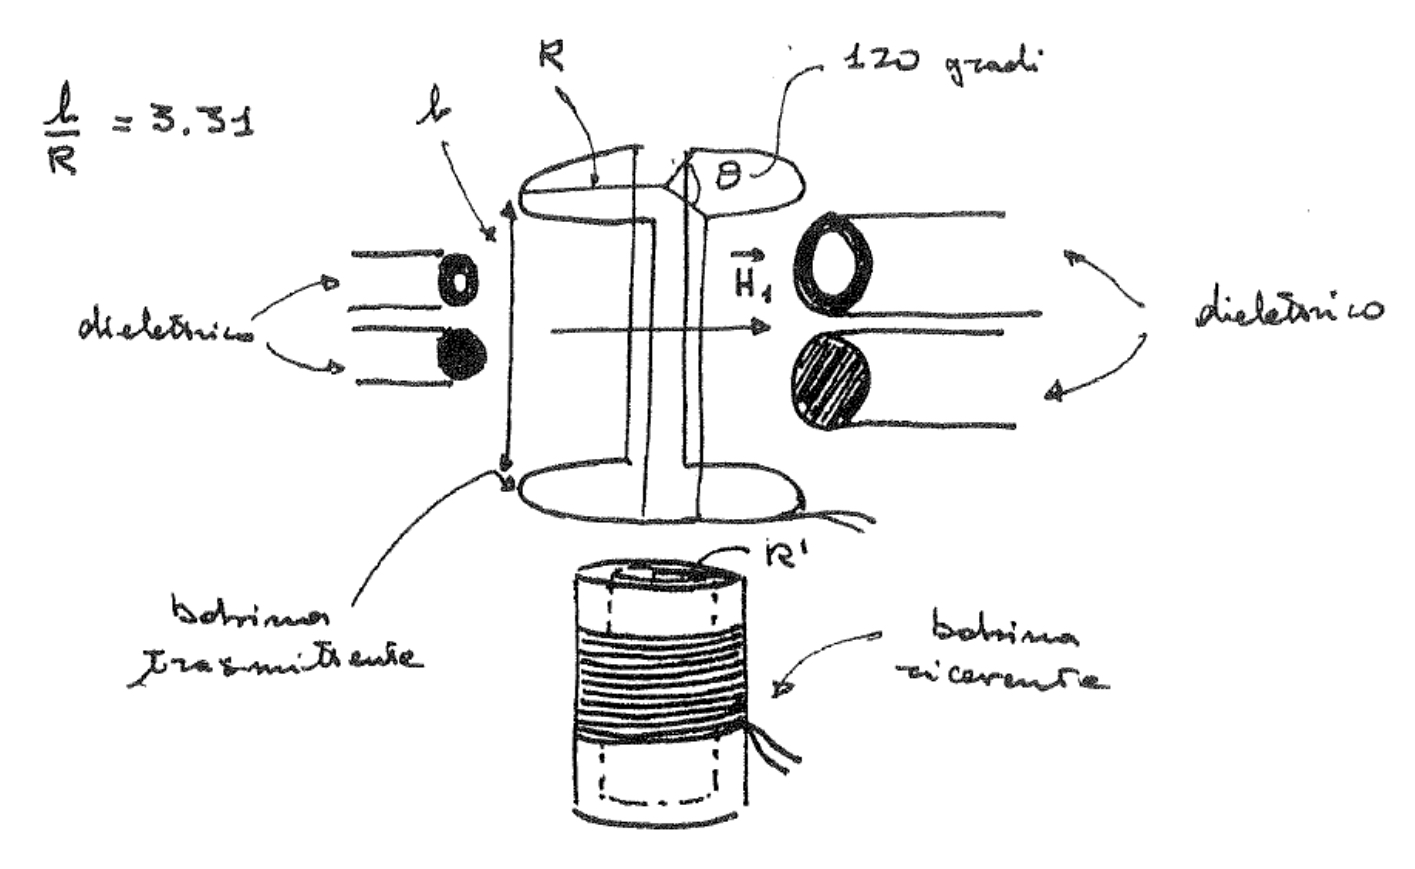
\includegraphics[trim={0cm 0 0 0},clip, width=0.49\textwidth]{probe} \end{wrapfigure}

Il coefficiente di riflessione del probe NMR mostra minimo  nella carta LogMag a \SI{-38.2}{\decibel} (Ref. \SI{-20}{\decibel})per \SI{32.1}{\mega\hertz} mentre il minimo del coefficiente di trasmissione a \SI{-86.1}{\decibel} (Ref \SI{-75}{\decibel}) per \SI{31.3}{\mega\hertz}.

\begin{figure}[!ht] \begin{subfigure}[b]{0.47\textwidth} \centering 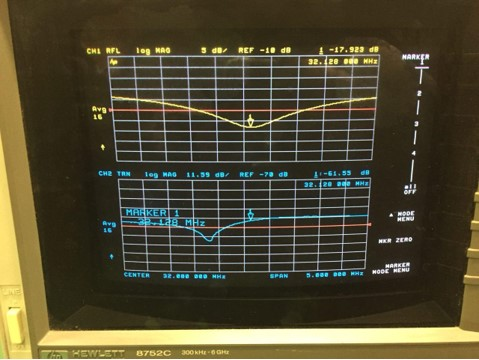
\includegraphics[trim={0cm 0 0 0},clip, width=0.47\textwidth]{probeR}\label{fig:probeR} \end{subfigure} ~ \begin{subfigure}[b]{0.47\textwidth} \centering 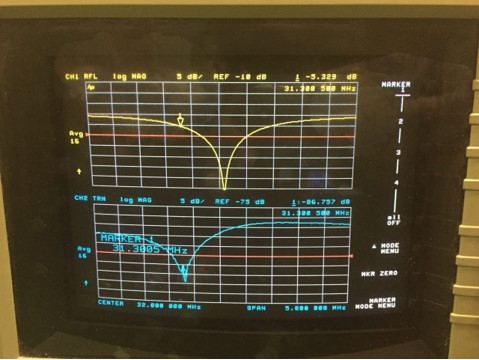
\includegraphics[trim={0cm 0 0 0},clip,width=0.47\textwidth]{probeT}\label{fig:probeT}
\end{subfigure} \end{figure} 


%\section{Rivelazione NMR}
%\begin{itemize}
%\item Tecniche passive in onda continua.
%Induzione di Bloch, Q meter, metodi a ponte.
%\item Tecniche attive in onda continua: oscillatori.
%Marginale, Robinson.
%\item Tecniche passive impulsive.
%\end{itemize} 
%\subsection{Linee trasmissione,}
%$V(x)=V_{i0}\exp{\gamma x}+V_{r0}\exp{\gamma x}$:
%\subsection{Ponte a T:}
%Frequenza per cui 
%\section{Ponti a T}

\pgfkeys{/pgf/fpu=false}

\end{document}
